\begin{acquis}
\begin{itemize}
\item BlaBla1
\item BlaBla2
\item BlaBla3
\item BlaBla4
\item BlaBla5
\item BlaBla6
\end{itemize}
\end{acquis}

\QCMautoevaluation{Pour chaque question, plusieurs réponses sont
  proposées.  Déterminer celles qui sont correctes.}

\begin{QCM}
  \begin{GroupeQCM}
    \begin{exercice}
       \renewcommand*\tabularxcolumn[1]{>{\centering\arraybackslash}m{#1}}
       \begin{ttableau}{0.35\linewidth}{8}
       \hline
       \cellcolor{A1} & \cellcolor{A1} & \cellcolor{A1} & \cellcolor{J1} &&&& \\\hline
       \cellcolor{J1} & \cellcolor{A1} & \cellcolor{J1} & \cellcolor{J1} &&&& \\\hline
       \cellcolor{J1} &&&&& \cellcolor{J1} & \cellcolor{J1} & \cellcolor{J1} \\\hline
       \end{ttableau}
      \begin{ChoixQCM}{4}
      \item Un tiers du rectangle est en orange
      \item $\dfrac{4}{20}$ du rectangle sont en bleu
      \item $\dfrac{8}{16}$ du rectangle sont en orange
      \item La moitié du rectangle est coloriée
      \end{ChoixQCM}
\begin{corrige}
     \reponseQCM{a} % j'ai mis "a" partout
   \end{corrige}
    \end{exercice}
    
    
    \begin{exercice}
      L'écriture décimale du quotient de 25 par 4 est \ldots
      \begin{ChoixQCM}{4}
      \item $\dfrac{25}{4}$
      \item $\dfrac{4}{25}$
      \item 6,25
      \item 0,16
      \end{ChoixQCM}
\begin{corrige}
     \reponseQCM{a} 
   \end{corrige}
    \end{exercice}
    
    
    \begin{exercice}
      $\dfrac{29}{7}$ est \ldots
      \begin{ChoixQCM}{4}
      \item égal à $4 + \dfrac{1}{7}$
      \item le nombre qui multiplié par 7 donne 29
      \item compris entre 4,1 et 4,2
      \item un nombre décimal
      \end{ChoixQCM}
\begin{corrige}
     \reponseQCM{a}
   \end{corrige}
    \end{exercice}
    
    
    \begin{exercice}
    
      \,\, \qquad \qquad 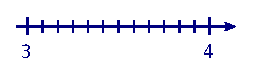
\includegraphics[width=4.2cm]{dd_34}
      
      Sur cette partie de demi‑droite graduée, on peut placer précisément \ldots
      \begin{ChoixQCM}{4}
      \item $3 + \dfrac{1}{11}$
      \item $2 + \dfrac{13}{12}$
      \item $\dfrac{11}{3}$
      \item $\dfrac{43}{12}$
      \end{ChoixQCM}
\begin{corrige}
     \reponseQCM{a}
   \end{corrige}
    \end{exercice}
 

    \begin{exercice}
      Sur la demi‑droite graduée ci‑dessous \ldots
      
      \qquad \qquad 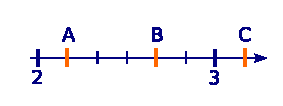
\includegraphics[width=4.2cm]{dd_ABC23}
      \begin{ChoixQCM}{4}
      \item $B$ a pour abscisse $\dfrac{4}{6}$
      \item $C$ a pour abscisse 4
      \item $A$ a pour abscisse \newline $2 + \dfrac{1}{6}$
      \item le point d'abscisse $\dfrac{5}{2}$ est entre $A$ et $B$
      \end{ChoixQCM}
\begin{corrige}
     \reponseQCM{a}
   \end{corrige}
    \end{exercice}
    
    
    \begin{exercice}
      $\dfrac{75}{20}$ est simplifiable par \ldots
      \begin{ChoixQCM}{4}
      \item 2
      \item 3
      \item 5
      \item 7
      \end{ChoixQCM}
\begin{corrige}
     \reponseQCM{a} 
   \end{corrige}
    \end{exercice}


    \begin{exercice}
      $\dfrac{12}{14}$ est égal à \ldots
      \begin{ChoixQCM}{4}
      \item $\dfrac{24}{48}$
      \item $\dfrac{112}{114}$
      \item $\dfrac{18}{21}$
      \item $\dfrac{6}{7}$
      \end{ChoixQCM}
\begin{corrige}
     \reponseQCM{a} 
   \end{corrige}
    \end{exercice}
    
    
    \begin{exercice}
      Les fractions que l'on peut encore simplifier sont \ldots
      \begin{ChoixQCM}{4}
      \item $\dfrac{1}{3}$
      \item $\dfrac{1\,765\,448}{267\,460}$
      \item $\dfrac{13}{26}$
      \item $\dfrac{987\,465}{34\,542\,290}$
      \end{ChoixQCM}
\begin{corrige}
     \reponseQCM{a} 
   \end{corrige}
    \end{exercice}
    
    
    \begin{exercice}
      $\dfrac{5}{8} = 0,625$ donc \ldots
      \begin{ChoixQCM}{4}
      \item $\dfrac{50}{80} = 0,625$
      \item $\dfrac{15}{18} = 0,625$
      \item $\dfrac{50}{8} = 6,25$
      \item $\dfrac{8}{5} = 0,625$      
      \end{ChoixQCM}
\begin{corrige}
     \reponseQCM{a} 
   \end{corrige}
    \end{exercice}
    \end{GroupeQCM}
\end{QCM}
 

\begin{QCM}
  \begin{GroupeQCM}
    \begin{exercice}
      $\dfrac{4}{3}$ est \ldots
      \begin{ChoixQCM}{4}
      \item $< 1$
      \item $> 1$
      \item $< \dfrac{2}{3}$
      \item $> \dfrac{3}{4}$
      \end{ChoixQCM}
\begin{corrige}
     \reponseQCM{a}
   \end{corrige}
    \end{exercice}
    
    
    \begin{exercice}
      $\dfrac{8}{15} \cdot 5 =$ \ldots
      \begin{ChoixQCM}{4}
      \item 2,6
      \item $\dfrac{40}{15}$
      \item $\dfrac{8}{3}$
      \item $\dfrac{8}{75}$
      \end{ChoixQCM}
\begin{corrige}
     \reponseQCM{a} 
   \end{corrige}
    \end{exercice}
    
    
    \begin{exercice}
      Prendre 25 \% d'un nombre, c'est \ldots
      \begin{ChoixQCM}{4}
      \item prendre le quart de ce nombre.
      \item multiplier ce nombre par $\dfrac{25}{100}$.
      \item diviser ce nombre par 4.
      \item ajouter 25 à \newline ce nombre.
      \end{ChoixQCM}
\begin{corrige}
     \reponseQCM{a}
   \end{corrige}
    \end{exercice}
    
    
    \begin{exercice}
      Pour calculer 37 \% de 600, on peut effectuer \ldots
      \begin{ChoixQCM}{4}
      \item $600 \div 37$
      \item $0,37 \cdot 600$
      \item $37 \cdot 6$
      \item $(600 \cdot 37) \div 100$
      \end{ChoixQCM}
\begin{corrige}
     \reponseQCM{a} 
   \end{corrige}
    \end{exercice}
 

    \begin{exercice}
      $\dfrac{2}{3} + \dfrac{2}{4} = \ldots$
      \begin{ChoixQCM}{4}
      \item $\dfrac{2}{7}$
      \item $\dfrac{4}{7}$
      \item $\dfrac{2}{3} + 2$
      \item $\dfrac{7}{6}$
      \end{ChoixQCM}
\begin{corrige}
     \reponseQCM{a} 
   \end{corrige}
    \end{exercice}


\end{GroupeQCM}
\end{QCM}

  